%\VignetteIndexEntry{Bootstrapped Feature Selection - Introduction}
%\VignetteDepends{}
%\VignetteKeywords{feature selection}
%\VignettePackage{bootfs}


\documentclass[11pt,a4paper]{article}

%\usepackage[round]{natbib}
\usepackage{amsmath}
\usepackage{amsfonts}
\usepackage{graphicx}
\usepackage[latin1]{inputenc}
\newcommand{\gene}[1]{\emph{#1}}

\setlength{\parskip}{1.5ex}
\setlength{\parindent}{0cm}

% NEW COMMANDS
% ------------------------------------------------
\newcommand{\Robject}[1]{\texttt{#1}}
\newcommand{\Rpackage}[1]{\textit{#1}}
\newcommand{\Rclass}[1]{\textit{#1}}
\newcommand{\Rfunction}[1]{{\small\texttt{#1}}}

\newcommand{\myincfig}[4]{
  \setkeys{Gin}{width=#1\textwidth}
  \begin{figure}[htbp]
    \begin{center}
      #2
      \caption{\label{#3}#4}
    \end{center}
  \end{figure}
  \setkeys{Gin}{width=.8\textwidth}
}


%%%%%%%%%%%%%%%%%%%%%%%%%%%%%%%%%%%%%%%%%%%%%%%%%%%%%
\usepackage{Sweave}
\begin{document}


\title{bootfs - Bootstrapped feature selection}
\author{ Christian Bender \footnote{Translational Oncology (TRON) Mainz, Germany. eMail: christian.bender@tron-mainz.de} }
\date{\today}
\maketitle


%\begin{abstract}
%\end{abstract}

This document describes the package 'bootfs' for robust feature selection in classification problems from high-throughput data, such as genomic or proteomic screening data. Several methods for classification are combined, in order to derive a robust estimation of the importance of each feature used for classification.

\section{Using bootfs}
\label{sec:quickstart}

This section contains the basic steps for analysis of high-throughput data, consisting of a number of samples to classify (such as patients) and a number of features, such as genes or proteins. Samples originate in two sample groups, for instance healthy versus sick patients. The aim is to find the most important features discriminating two or more classes within sample populations.

The usage of the package is illustrated for three classification algorithms: \emph{pamr} (Prediction analysis for Microarrays, \cite{Tibshirani2002}, implementation in \emph{pamr}-R-package), \emph{rf\_boruta} (Random forests with the Boruta algorithm for feature selection, \cite{Kursa2010}, implementation in \emph{Boruta}-R-package) and \emph{scad} (Support Vector Machines with Smoothly Clipped Absolute Deviation feature selection, \cite{Zhang2006}, implementation in the \emph{penalizedSVM} R-package \cite{Becker2011}). Also available feature selection methods (through \emph{penalizedSVM} package) are \emph{1norm} for L1-penalisation (LASSO), \emph{scad+L2} for Elastic-SCAD  and \emph{DrHSVM} for Elastic Net. Further, the original random forest implementation (\emph{randomForest}-R-package \cite{Breiman2001}) is available as method \emph{rf}, as well as the gradient boosting machine (\cite{Friedman2001,Friedman2002}) from package \emph{gbm} as method \emph{gbm}. The methods \emph{pamr}, \emph{rf}, \emph{rf\_boruta} and \emph{gbm} also allow multi-class classification. First of all load the package:

%% chunk 1
\begin{Schunk}
\begin{Sinput}
> library(bootfs)
\end{Sinput}
\end{Schunk}


\subsection{Simulating data}
Data can be simulated using a built in function \emph{simDataSet}. This samples a data matrix with \emph{nsam} samples and \emph{ngen} genes, as well as a grouping vector defining two sample groups.

\begin{Schunk}
\begin{Sinput}
> set.seed(1234)
> data <- simDataSet(nsam=30, ngen=100, sigma=1.5, plot=TRUE)
> logX <- data$logX
> groupings <- data$groupings
\end{Sinput}
\end{Schunk}

\subsection{Assessing performance of the classifiers}

The first step is to verify, if the feature selection algorithms perform sufficienctly on the given data set. For this, a crossvalidation of different classification algorithms is run:

\begin{Schunk}
\begin{Sinput}
> ## run the crossvalidation
> ## note the number of repeats should be set to 10 or so, 
> ## it is set to 2 here to have a low running time of this illustration
> ## create a parameter object used for the different methods
> # for crossvalidation
> paramsCV <- control_params(seed=123,
+  ncv=5, repeats=2, jitter=FALSE,      ## general parameters
+  maxiter=100, maxevals=50,             ## svm parameters
+  max_allowed_feat=500, n.threshold=50, ## pamr parameters
+  maxRuns=300,                          ## RF parameters
+  ntree = 1000,                         ## GBM parameters
+  shrinkage = 0.01, interaction.depth = 3,
+  bag.fraction = 0.75, train.fraction = 0.75, 
+  n.minobsinnode = 3, n.cores = 1, 
+  verbose = TRUE)
> ## run the crossvalidation
> ## takes a while
> methods <- c("pamr", "scad", "rf_boruta")
> retCV <- doCV(logX, groupings, fs.methods = methods, DIR = NULL, params=paramsCV)
\end{Sinput}
\end{Schunk}

The above command uses the classification methods PAMR, SCAD-SVM and RF-Boruta and performs a 5-fold (ncv=5) crossvalidation on the training data, repeating the crossvalidation 2 times with different training/test set assignments. Classification methods and k-fold for the CV can be easily exchanged by setting the appropriate parameters. The results of the crossvalidation are summarised as ROC (Receiver operator characteristic) curves together with the corresponding AUC (area under the curve), shown in figures \ref{fig:rocpam}, \ref{fig:rocrf} and \ref{fig:rocscad}.

\begin{figure}[htp]
\centering
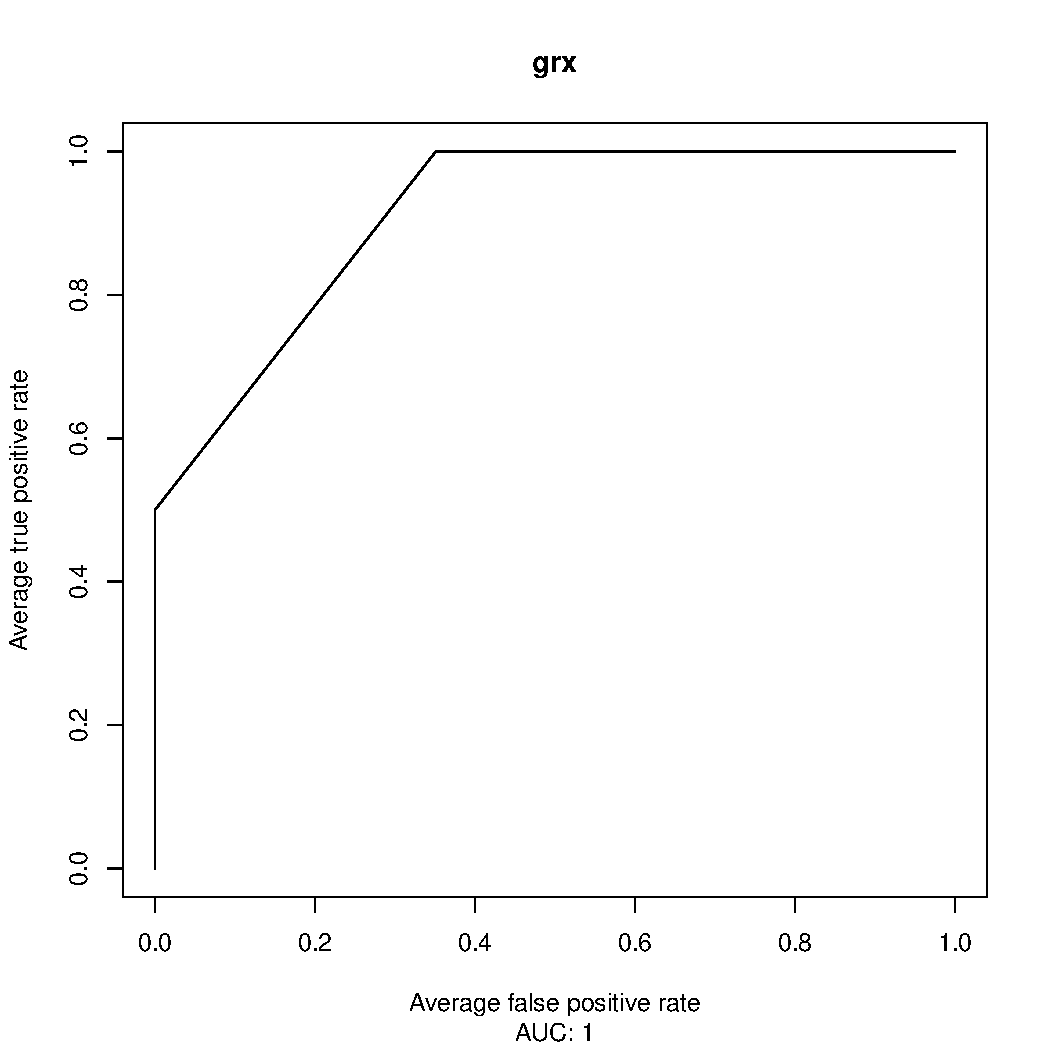
\includegraphics[width=8cm,height=8cm]{rocpam}
\caption{Receiver Operator Characteristic (ROC) curve for the PAM algorithm cross-validation. Input data were the simulated data matrix and grouping vectore for 30 samples and 100 features.}
\label{fig:rocpam}
\end{figure}

\begin{figure}[htp]
\centering
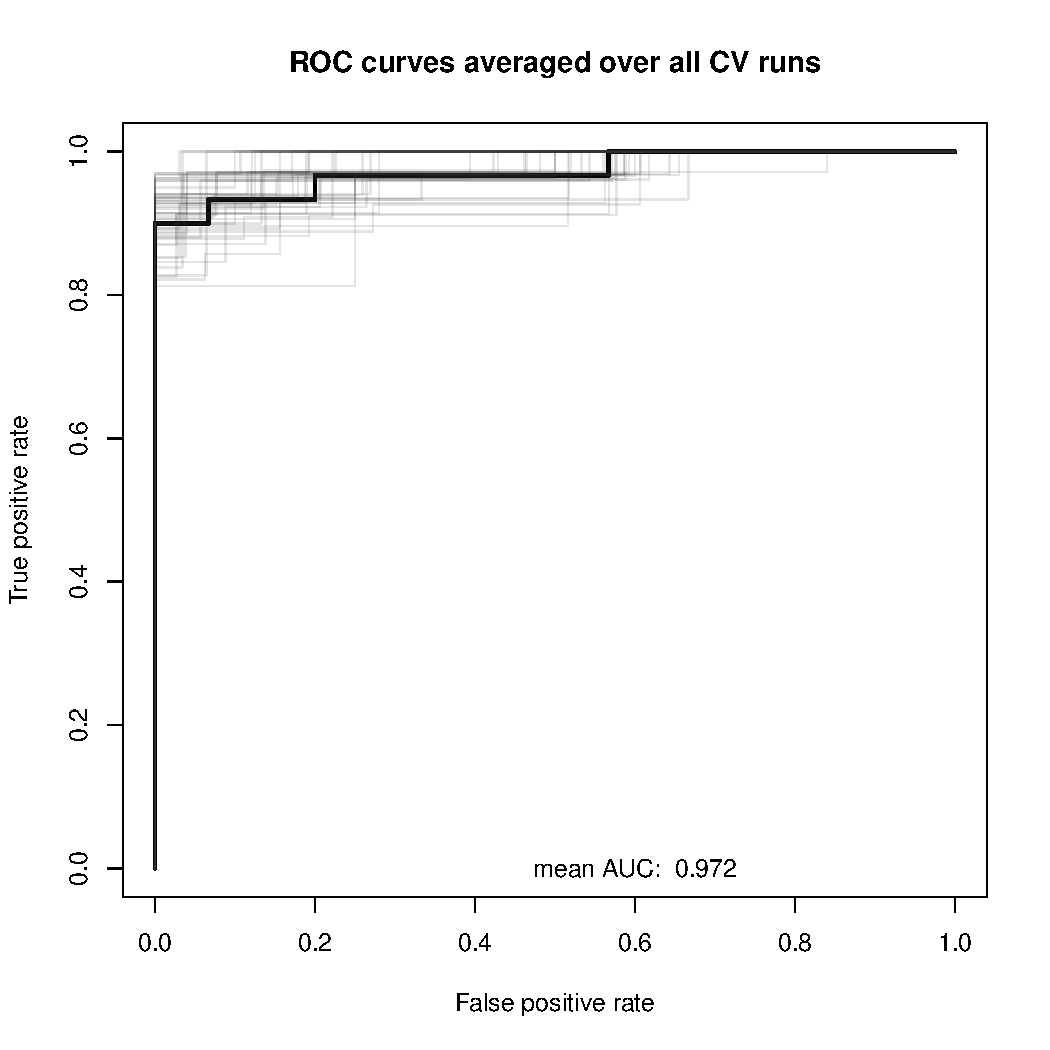
\includegraphics[width=8cm,height=8cm]{rocrf}
\caption{Receiver Operator Characteristic (ROC) curve for the random forest RF-Boruta algorithm cross-validation. Input data were the simulated data matrix and grouping vectore for 30 samples and 100 features.}
\label{fig:rocrf}
\end{figure}

\begin{figure}[htp]
\centering
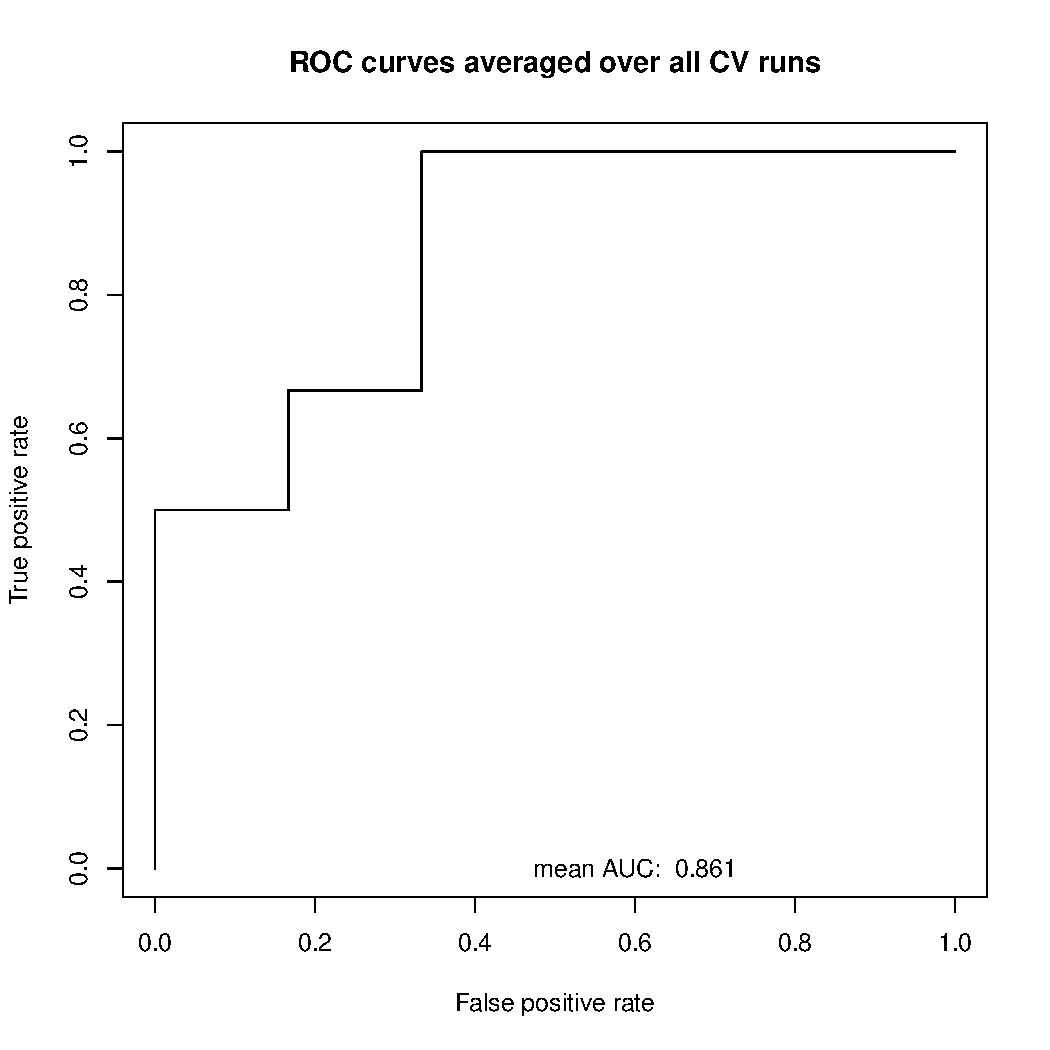
\includegraphics[width=8cm,height=8cm]{rocscad}
\caption{Receiver Operator Characteristic (ROC) curve for the SCAD-SVM algorithm cross-validation. Input data were the simulated data matrix and grouping vectore for 30 samples and 100 features.}
\label{fig:rocscad}
\end{figure}



\subsection{Do the feature selection and importance ranking}

If the performance is of sufficient quality, as seen in the ROC curves generated during the cross-validation, the bootstrapping approach for deriving the most important features for this classification task can be done. Again, we select the three algorithms from above and perform bootstrapping on the input data. For each bootstrapping data set the feature selections are done using each algorithm. 

\begin{Schunk}
\begin{Sinput}
> # for bootstrapping
> paramsBS <- control_params(seed=123,
+  jitter=FALSE, bstr=15,                  ## general parameters
+  maxiter=100, maxevals=50, bounds=NULL,  ## svm parameters
+  max_allowed_feat=500, n.threshold=50,   ## pamr parameters
+  maxRuns=300,                            ## RF parameters
+  ntree = 1000,                           ## GBM parameters
+  shrinkage = 0.01, interaction.depth = 3,
+  bag.fraction = 0.75, train.fraction = 0.75, 
+  n.minobsinnode = 3, n.cores = 1, 
+  verbose = TRUE, saveres=FALSE
+ )
> ## run the bootstrapping
> ## takes a while
> methods <- c("pamr", "scad", "rf_boruta")
> retBS <- doBS(logX, groupings, fs.methods=methods, DIR="bs", params=paramsBS)
> 
\end{Sinput}
\end{Schunk}

Here, 15 bootstrap sample sets are drawn (bstr=15) and feature Selection is done for each sample set. The group proportions are kept constant during the sample selection. Now, for each method, a separate importance graph can be generated:

\begin{Schunk}
\begin{Sinput}
> ## show an importance ranking for a single 
> ## classification method
> bsres <- makeIG(retBS[[1]], SUBDIR=NULL, prob=.999)
\end{Sinput}
\end{Schunk}

This might be useful to inspect the selected features for each method separately. The parameter \emph{prob=.9} is used to define the cutoff value, how often a feature at least must co-occur with another feature, in which case an edge is drawn between them. However, the general ranking of the importance of the features is done by generating the combined importance graph from all selected methods:

\begin{Schunk}
\begin{Sinput}
> ## create the combined importance graph for all methods
> ## and export the adjacency matrix containing the 
> ## numbers of occuerrences of the features, as well 
> ## as the top hits.
> res <- resultBS(retBS, DIR=NULL, vlabel.cex = 3, filter = 5)
\end{Sinput}
\end{Schunk}

There are several arguments which customise the look of the importance graph. In this call, the \emph{vlabel.cex} argument defines the magnification factor of the node labels (each node corresponds to one feature). The argument \emph{filter} can be used to specify, how often a feature must co-occur with another, such that an edge is drawn between the two features. Figure \ref{fig:impgraph1} shows the result of the above call.

\begin{figure}[htp]
\centering
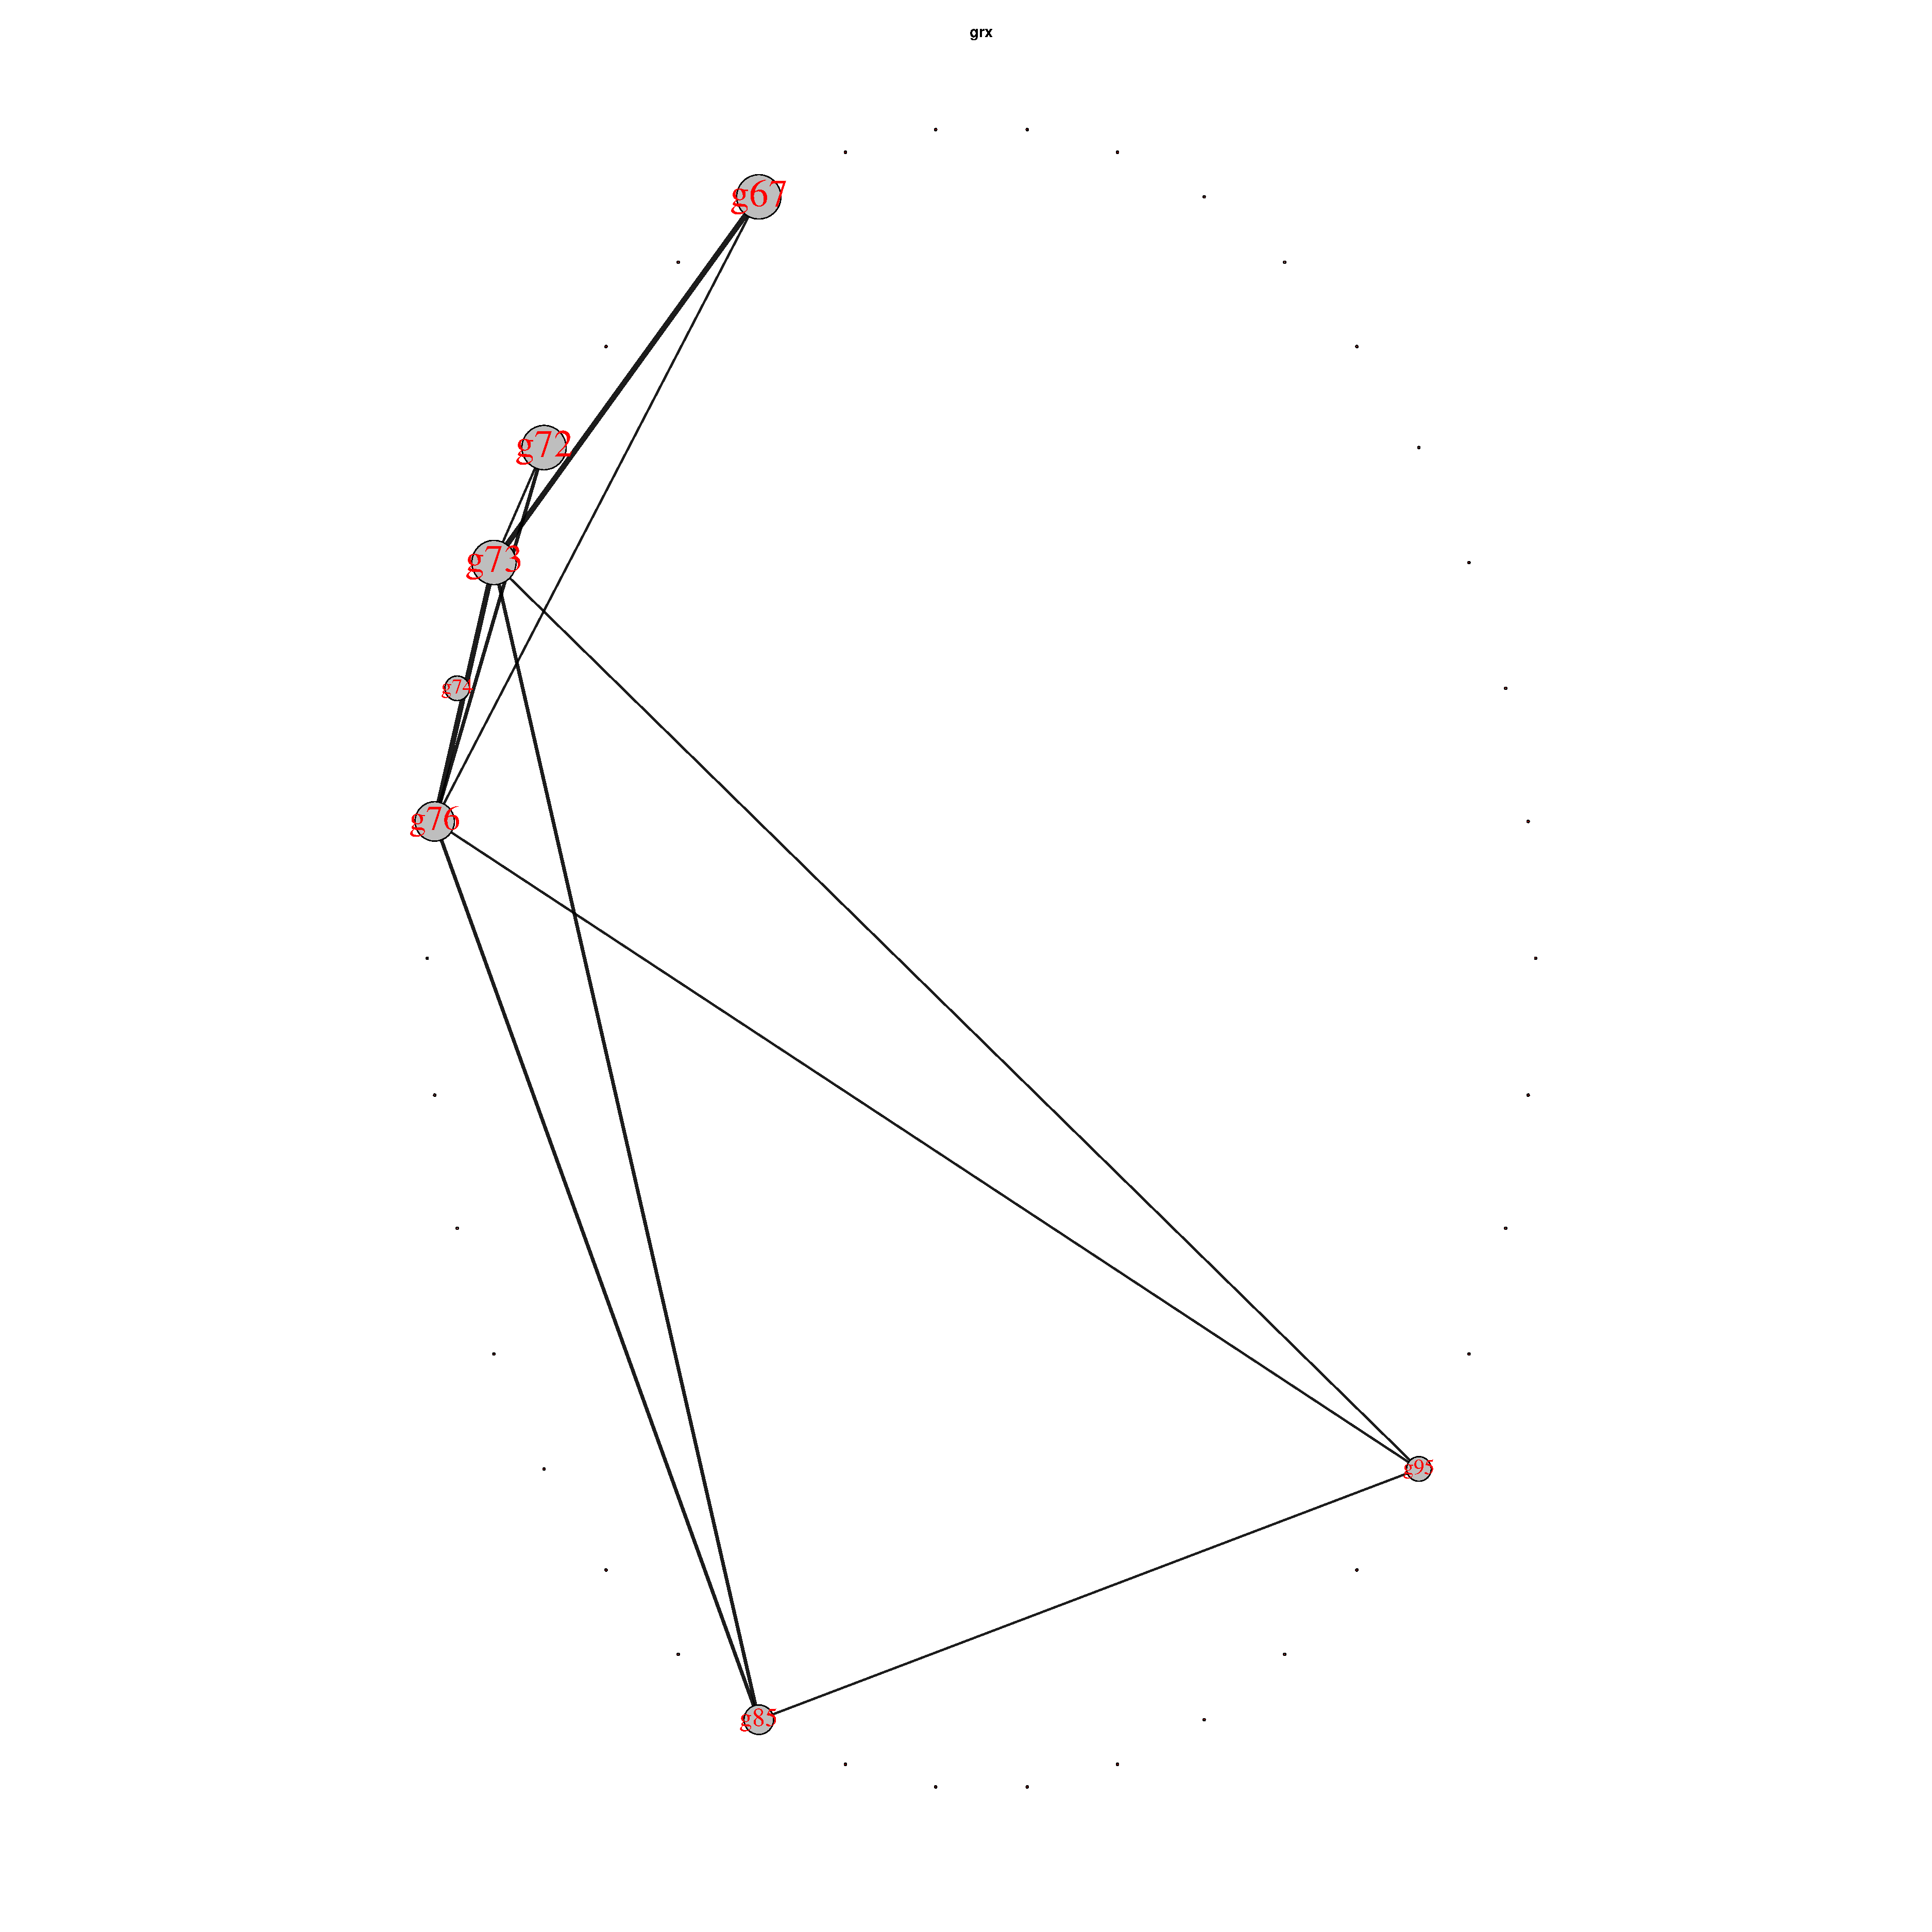
\includegraphics[width=12cm,height=12cm]{impgraph1}
\caption{Importance graph generated by \emph{resultBS}. Node width is proportional to the absolute frequency of occurrence of a feature across all bootstrap feature selections. Edge width is proportional to the frequency of co-occurrence of the two adjacent nodes.}
\label{fig:impgraph1}
\end{figure}

The graph can be customised more flexibly using the \emph{importance\_igraph} function directly:

%  pdf("impgraph2.pdf", width=10, height=10)
\begin{Schunk}
\begin{Sinput}
> ## plot the importance graph directly. Gives more 
> ## flexibility to adjust the graph
> 
> resx <- res[[1]]
> ig <- importance_igraph(resx$adj, main = "my test", 
+  highlight = NULL,	layout="layout.ellipsis",
+  pdf=NULL, pointsize=12, tk=FALSE,
+  node.color="grey", node.filter=NULL,
+  vlabel.cex=2, vlabel.cex.min=0.5, vlabel.cex.max=5,
+  max_node_cex=8,
+  edge.width=2, edge.filter=2, max_edge_cex=5, ewprop=3 )       
\end{Sinput}
\end{Schunk}

% dev.off()

Figure \ref{fig:impgraph2} shows the importance graph generated with the above call. Arguments \emph{vlabel.cex}, \emph{vlabel.cex.min} and \emph{vlabel.cex.max} can be used to adjust the overall, minimum and maximum expansion factor for the node labels. \emph{max\_node\_cex} controls the maximum expansion factor of the node size. The size of the nodes is always proportional to the absolute occurrence of the feature in the \emph{bstr} bootstrapping sample sets. \emph{edge.width} and \emph{max\_edge\_cex} are used for setting the edge width and expansion factor for the edges, respectively, while \emph{ewprop} is a proportionality factor controlling the decrease of edge width with decreasing frequency. A higher value of \emph{ewprop} means a fast reduction of edge width and thus a less densly packed importance graph plot. Also consider the help pages for the respective functions, to learn about the remaining function arguments.

\begin{figure}[htp]
\centering
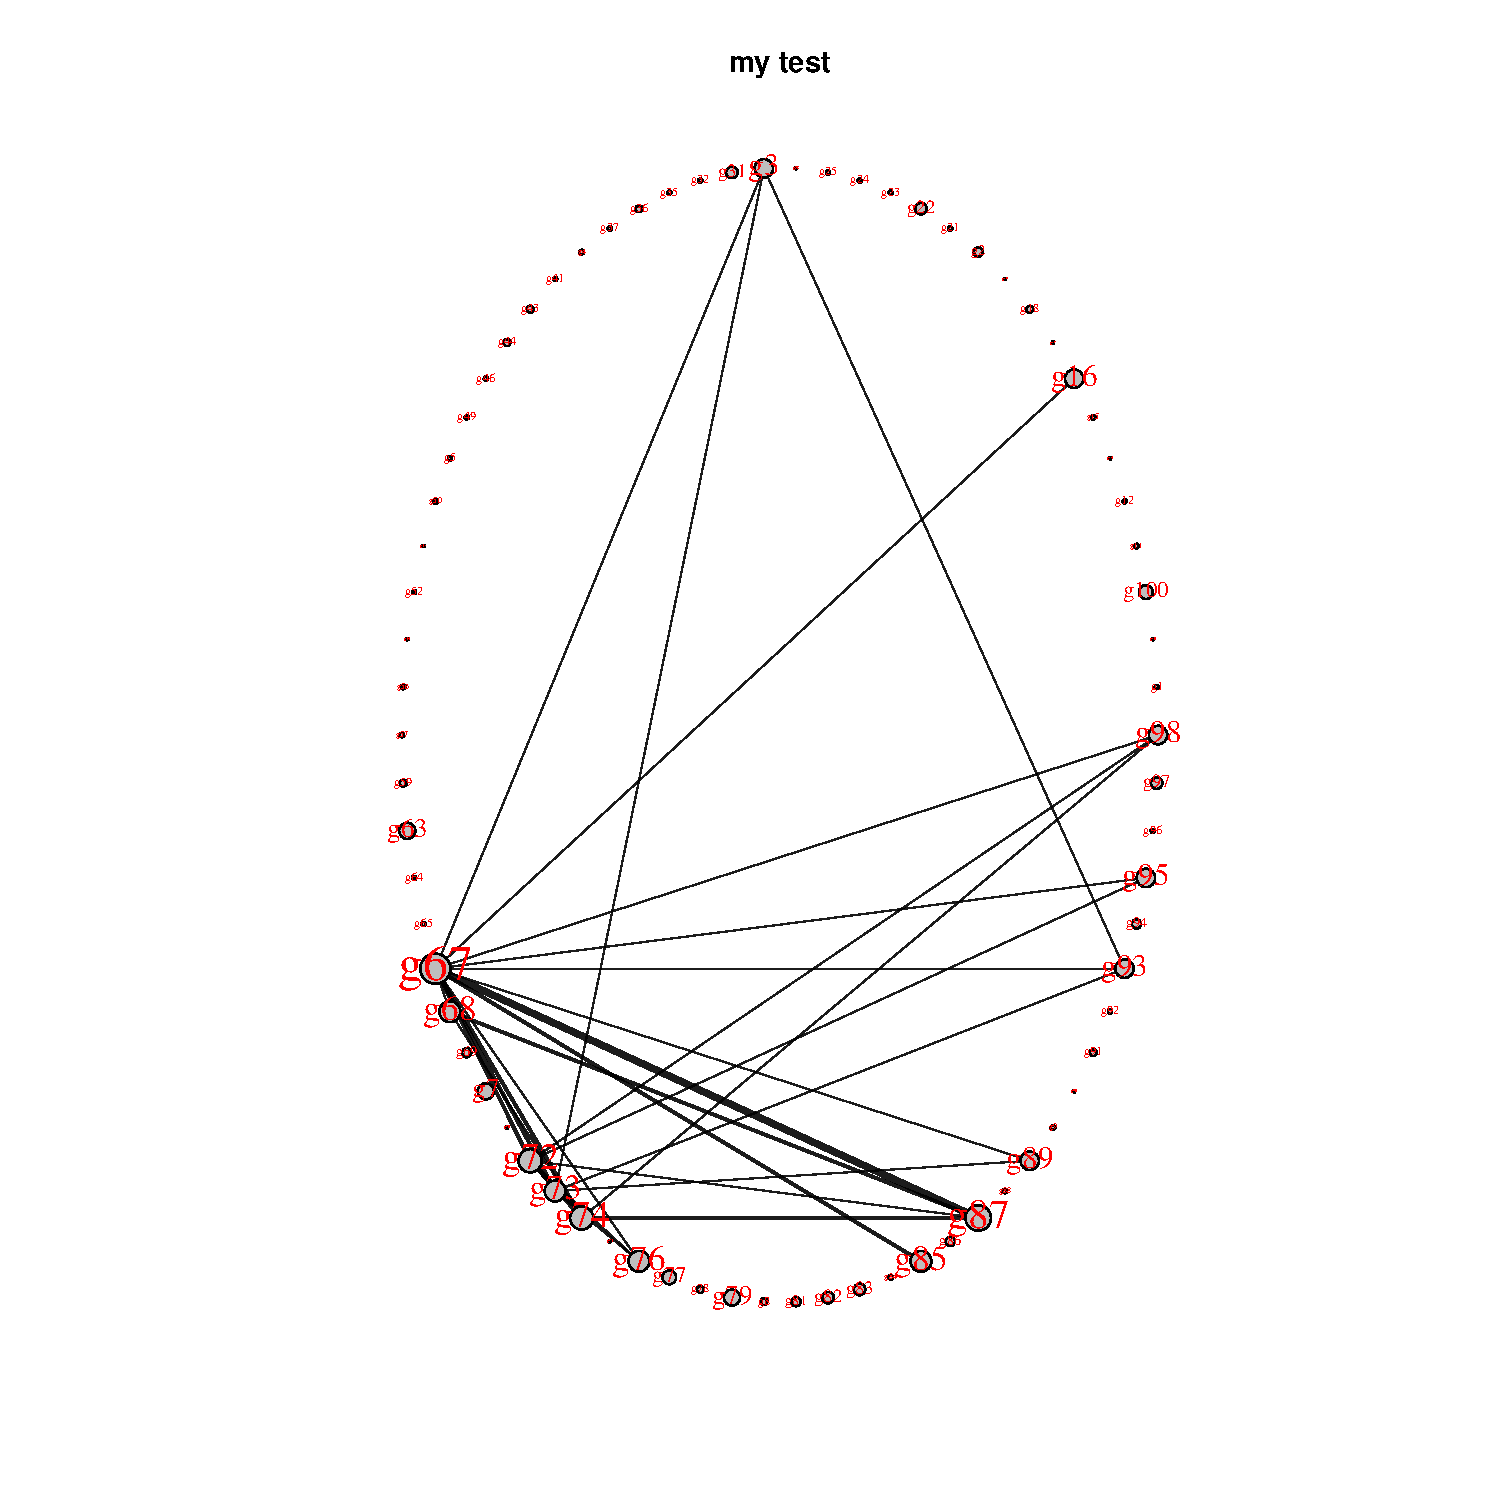
\includegraphics[width=10cm,height=10cm]{impgraph2}
\caption{Importance graph generated by call to \emph{importance\_igraph} directly. Note how the edge widths are thicker but decreasing more rapidly as in figure \ref{fig:impgraph1}, achieved by setting \emph{max\_edge\_cex} and \emph{ewprop} appropriately. Besides, the node label sizes are adjusted using \emph{vlabel.cex}.}
\label{fig:impgraph2}
\end{figure}


%\begin{scriptsize}
%\begin{table}[h]
%\begin{tiny}
%\label{tab:exampledatamatrix}
%\begin{tabular}{l|cccccccc}
%	& EGF\_1& EGF\_1 & EGF\_2 & EGF\_2 & EGF\&X\_1 & EGF\&X\_1 & %EGF\&X\_2 & EGF\&X\_2\\
%	\hline
%	EGF & 0 &  0 &  0  & 0 &  0 &  0  & 0 &  0 \\
%	X   & 0 &  0 &  0  & 0  & 0 & 0 &  0  & 0 \\
%	AKT & 1.45 & 1.8 &  0.99 & 1.6 & 1.78 & 1.8  & 1.56 & 1.58 \\
%	ERK & 1.33 & 1.7 &  1.57 & 1.3  & 0.68 & 0.34 & 0.62 & 0.47 \\
%	MEK & 0.45 & 0.8 &  0.99 & 0.6  & 0.78 & 0.8  & 0.56 & 0.58
%\end{tabular}
%\caption{Example data matrix for 3 nodes and 2 stimuli.}
%\end{tiny}
%\end{table}

%\end{scriptsize}

\subsection{Doing multi-class classification}

It is also possible to classify multiple classes at once. To illustrate this, we show an analysis of Fisher's Iris Data set. The goal is to discriminate between three Iris species (\emph{Iris setosa}, \emph{Iris virginica} and \emph{Iris versicolor}), using four features \emph{Sepal length, Sepal width, Petal length and Petal width}. We load the Iris data set and prepare it for bootfs:

\begin{Schunk}
\begin{Sinput}
> ## do multiclass classification
> ## load the data
> data(iris)
> groupings <- list(Species=iris$Species)
> logX <- iris[,1:4]
> methods <- c("gbm","rf","pamr")
> paramsCV <- control_params(seed=123,
+  ncv=5, repeats=2, jitter=FALSE,      ## general parameters
+  maxiter=100, maxevals=50,             ## svm parameters
+  max_allowed_feat=500, n.threshold=50, ## pamr parameters
+  maxRuns=300,                          ## RF parameters
+  ntree = 1000,                         ## GBM parameters
+  shrinkage = 0.01, interaction.depth = 3,
+  bag.fraction = 0.75, train.fraction = 0.75, 
+  n.minobsinnode = 3, n.cores = 1, 
+  verbose = TRUE)
\end{Sinput}
\end{Schunk}

Here we use the Gradient Boosting Machine, Breiman's Random Forests and PAMR. As usual we perform a crossvalidation of the selected methods, to assess their individual performance:

\begin{Schunk}
\begin{Sinput}
> ## crossvalidation
> retCV <- doCV(logX, groupings, fs.methods = methods, DIR = NULL, params=paramsCV)
\end{Sinput}
\end{Schunk}

A summary of the CV results can be obtained using the \emph{resultsCV} function:

% pdf("resultcvmulti.pdf",width=6,height=6, pointsize=16)
 
\begin{Schunk}
\begin{Sinput}
> resultCV(retCV)
\end{Sinput}
\end{Schunk}

% dev.off()

\begin{figure}[htp]
\centering
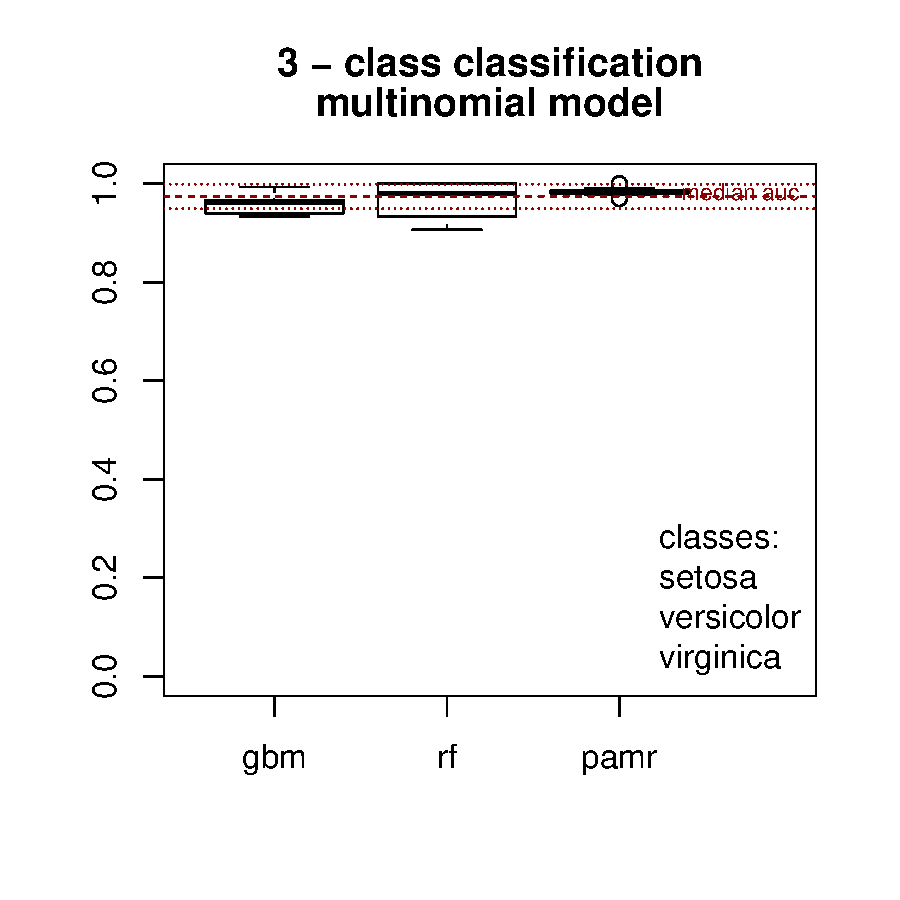
\includegraphics[width=6cm,height=6cm]{resultcvmulti}
\caption{Multiclass AUCs generated with the \emph{pROC} package. Shown are the distributions of AUCs over all cross-validation repeats and folds.}
\label{fig:resultcv}
\end{figure}

Note that ROC curve display is not possible for more than two classes. For assessment of the performance we rely on the area under curve calculation for multiclass problems \cite{Robin2011}, implemented in the \emph{pROC} package. this gives us the AUC for each CV fold and repeat.\\


Now, we can proceed to the bootstrapped feature selection:

\begin{Schunk}
\begin{Sinput}
> paramsBS <- control_params(seed=123,
+  jitter=FALSE, bstr=15,                  ## general parameters
+  maxiter=100, maxevals=50, bounds=NULL,  ## svm parameters
+  max_allowed_feat=500, n.threshold=50,   ## pamr parameters
+  maxRuns=300,                            ## RF parameters
+  ntree = 1000,                           ## GBM parameters
+  shrinkage = 0.01, interaction.depth = 3,
+  bag.fraction = 0.75, train.fraction = 0.75, 
+  n.minobsinnode = 3, n.cores = 1, 
+  verbose = TRUE, saveres=FALSE
+ )
> ## bootstrapped feature selection
> retBS <- doBS(logX, groupings, fs.methods=methods, DIR=NULL, params=paramsBS)
\end{Sinput}
\end{Schunk}

The results are generated and the importance graph is plotted:

% pdf("resultbsmulti.pdf",width=12,height=8, pointsize=16)

\begin{Schunk}
\begin{Sinput}
> ## make results from all methods used
> res <- resultBS(retBS, DIR=NULL, vlabel.cex = 3, filter = 1)
> ## plot the importance graph
> resx <- res[[1]]
> ig <- importance_igraph(resx$adj, main = "multiclass test, IRIS data", 
+         highlight = NULL,	layout="layout.ellipsis",
+ 		pdf=NULL, pointsize=12, tk=FALSE,
+ 		node.color="grey", node.filter=NULL,
+ 		vlabel.cex=1.2, vlabel.cex.min=0.5, vlabel.cex.max=4,
+ 		max_node_cex=8,
+         edge.width=1, edge.filter=1, max_edge_cex=2, ewprop=3 )
\end{Sinput}
\end{Schunk}

% dev.off()

\begin{figure}[htp]
\centering
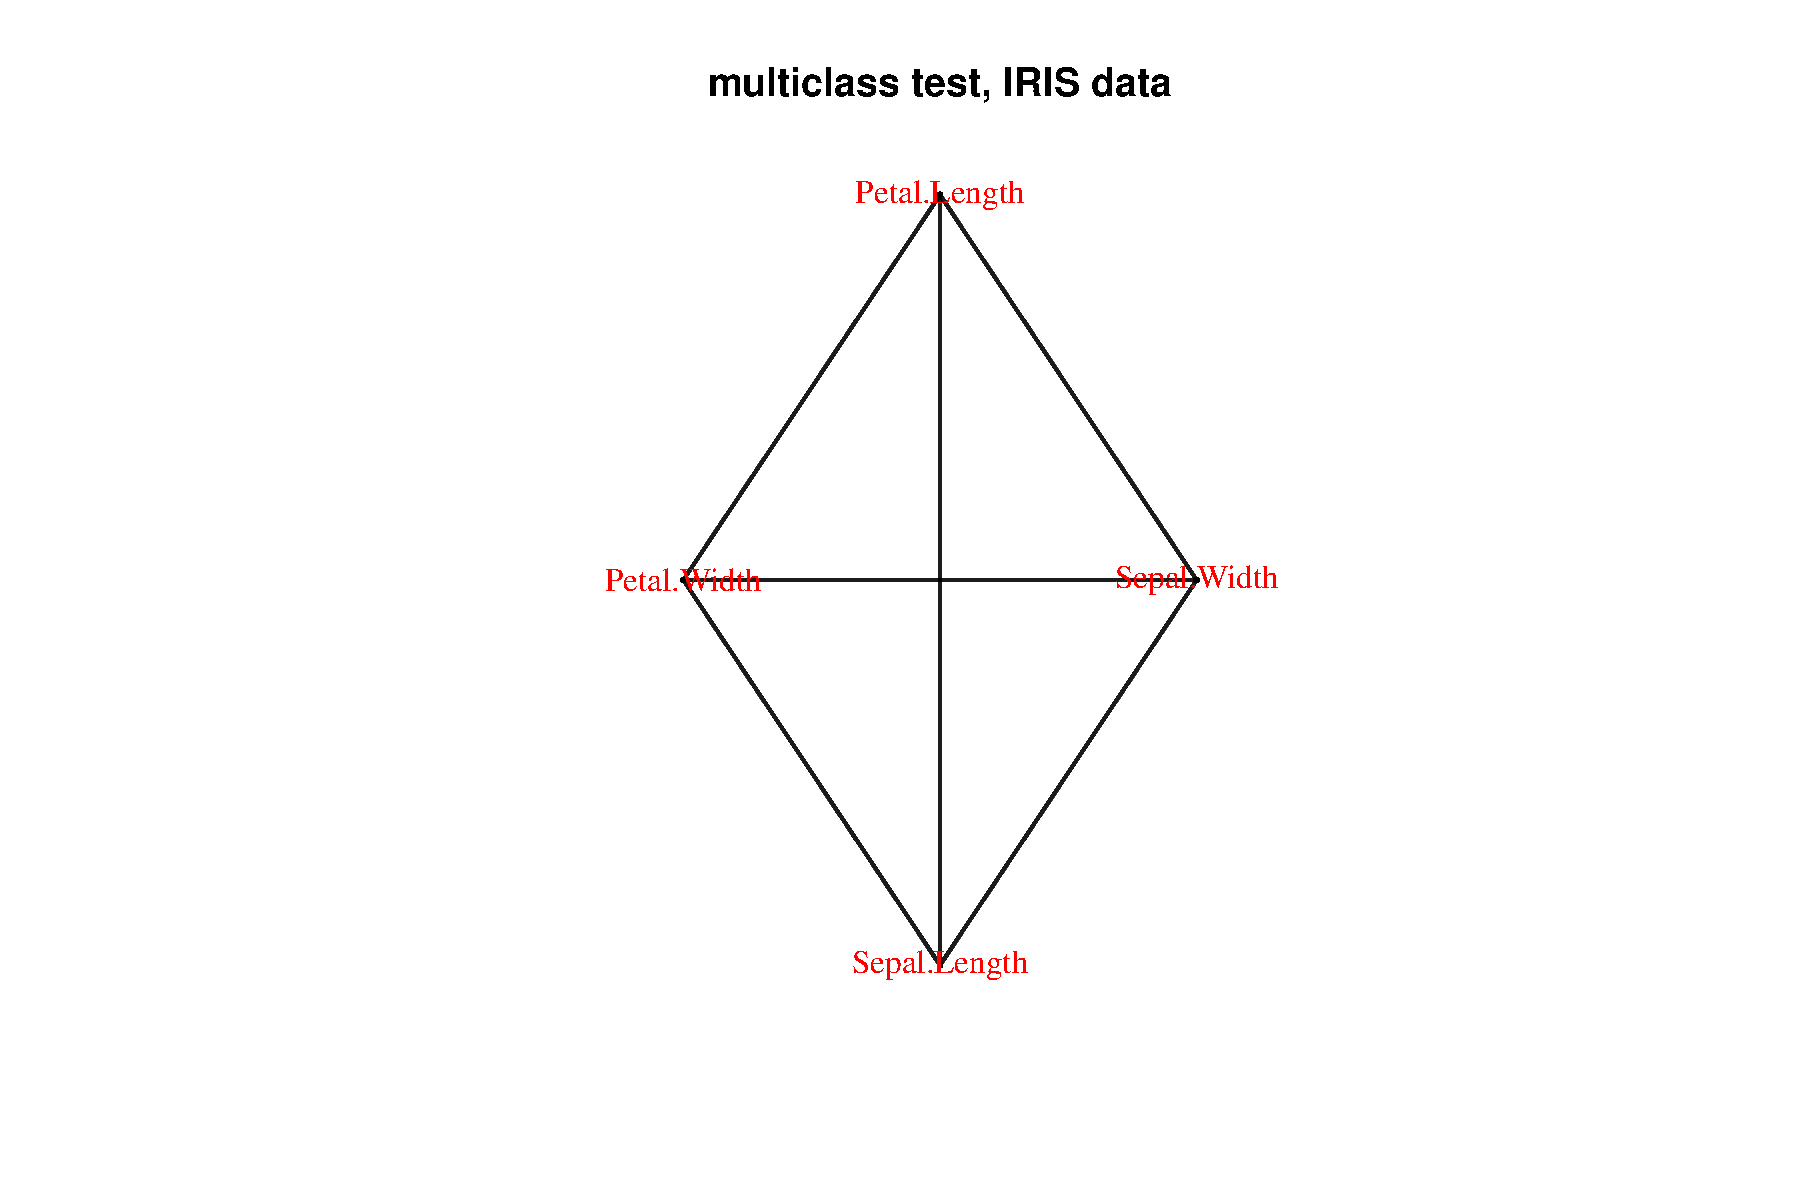
\includegraphics[width=8cm,height=6cm]{resultbsmulti}
\caption{Result of multiclass bootfs, done on the IRIS data set. All 4 features are left.}
\label{fig:resultbs}
\end{figure}


\clearpage

\section*{Session Information}

The version number of R and packages loaded for generating the vignette were:


\begin{itemize}\raggedright
  \item R version 3.0.2 RC (2013-09-17 r63939), \verb|x86_64-unknown-linux-gnu|
  \item Locale: \verb|LC_CTYPE=en_US.UTF-8|, \verb|LC_NUMERIC=C|, \verb|LC_TIME=en_US.UTF-8|, \verb|LC_COLLATE=C|, \verb|LC_MONETARY=en_US.UTF-8|, \verb|LC_MESSAGES=en_US.UTF-8|, \verb|LC_PAPER=en_US.UTF-8|, \verb|LC_NAME=C|, \verb|LC_ADDRESS=C|, \verb|LC_TELEPHONE=C|, \verb|LC_MEASUREMENT=en_US.UTF-8|, \verb|LC_IDENTIFICATION=C|
  \item Base packages: base, datasets, grDevices, graphics, methods,
    stats, utils
  \item Loaded via a namespace (and not attached): tools~3.0.2
\end{itemize}
\bibliographystyle{plain}  % Style BST file
\bibliography{references}     % Bibliography file (usually '*.bib' ) 
\end{document}

%
%   end of file
%
%%%%%%%%%%%%%%%%%%%%%%%%%%%%%%%%%%%%%%%%%%%%%%%%%%%%%%%%%%%%%%%%%%%%%%%%%%%%%%%%
